\chapter{Approach}
\label{sec:approach}
\section{From Images to Time Series}
\label{sec:from images to time series}
After establishing a solid foundation regarding the inner workings of DDPM in section \ref{sec:ddpm}, this knowledge was applied to define the necessary operations and methods. This enabled the construction of a working DDPM for testing and evaluation.\newline
Very beneficial is the fact, that the overall mathematical semantic of the equations described in \ref{sec:ddpm} does not need to be changed
just some technical changes to the shapes of the matrices, that are multiplied, to guarantee the right output forms was made.
After incorporating these changes the forward process could be performed and visualized as seen in fig. \ref{fig:time series ddpm process}.
Using images the forward process or the noising of an image can be understood intuitively. The same effect can now be achieved by looking at the
noised time series. The last step if the noising process resembles just random noise, while the intermediate steps still hold some characteristics.\newline
After establishing the forward process noised sampling can be performed which empowers us to define an 
efficient training cycle. Before a model is trained, the first step involves defining the underlying architecture that will predict the noise used in the backward process.
\begin{figure}
    \centering
    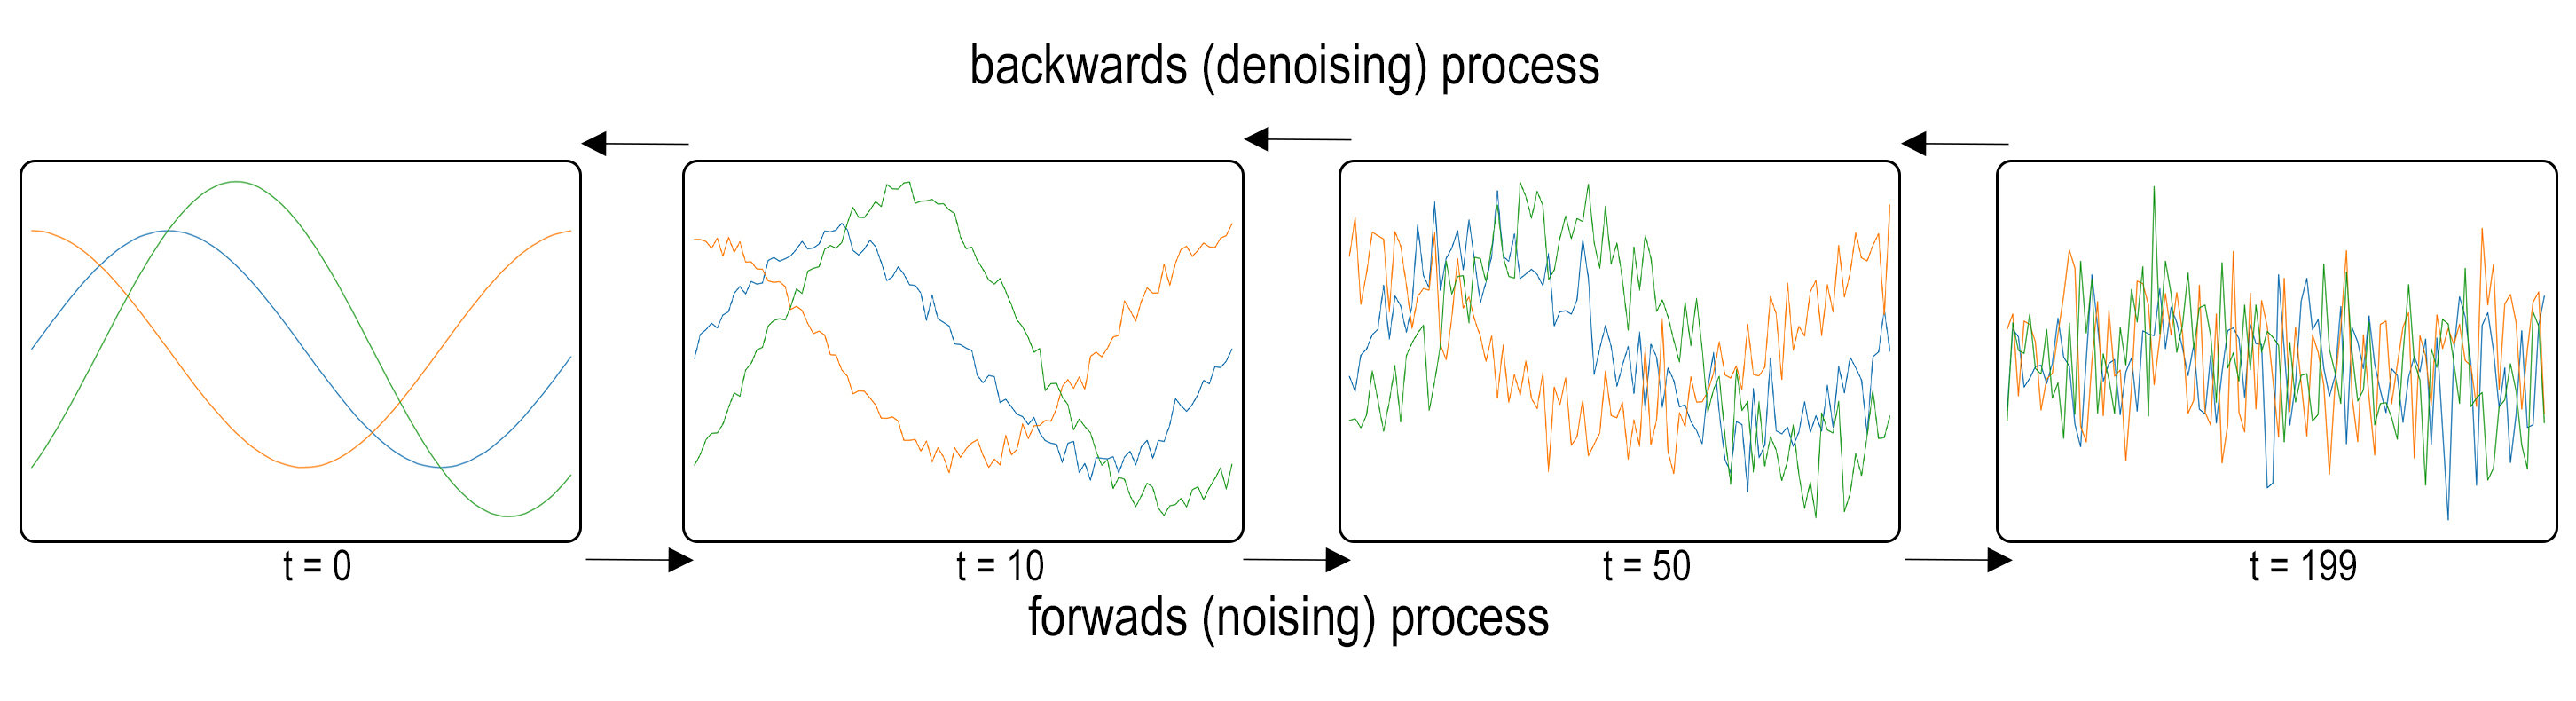
\includegraphics[width=\textwidth]{images/noised time series.jpg}
    \caption{Visualization of the forward/backwards process of a DDPM for time series samples with T = 200 using different sin/cos waves.}
    \label{fig:time series ddpm process}
\end{figure}
\section{UNET for Time Series}
\label{sec:unet time series}
The UNET architecture, as described in \ref{sec:unet}, was taken, and it was restructured to function with 1-D time series data. Mostly, this was achieved by replacing 2-D convolutional and 2-D transposed convolutional 
layers with the corresponding 1-D variants. The underlying structure of our UNET can be visualized by figure \ref{fig:unet} just that it takes 1D input samples instead of 2D images as already mentioned.\newline
After establishing the base structure, additions to the UNET that differ from the original setup are also defined. One of those
additions are self attention layers after every up-/downsampling block. Also these blocks take an extra parameters
as input - a timestamp. This is the timestamp that is defined in the DDPM operations in section \ref{sec:ddpm}. Before going into the UNET this timestamp
is positionally encoded. After that the timestamp is embedded linearly in the convolutions. So in every up-/downsampling block the model retains information about the current step in the noising/denoising process.\newline
Conditional dependencies in the form of an entity embedding \cite{guo2016entity} were also added to the UNET. This embedding allows us to embed categorical and continual information that can also be provided to the UNET to guarantee
a more controlled generative process. The model can produce samples that correspond to a specific time of the year or resemble certain sample features like average temperature. The embedding dimensions are chosen in a way so that the 
dimension of the positional encoding of the timestamp match. Those two embeddings are added afterwards to form a new timestamp that now also holds contextual information about the sample in every block. 
\begin{figure}
    \centering
    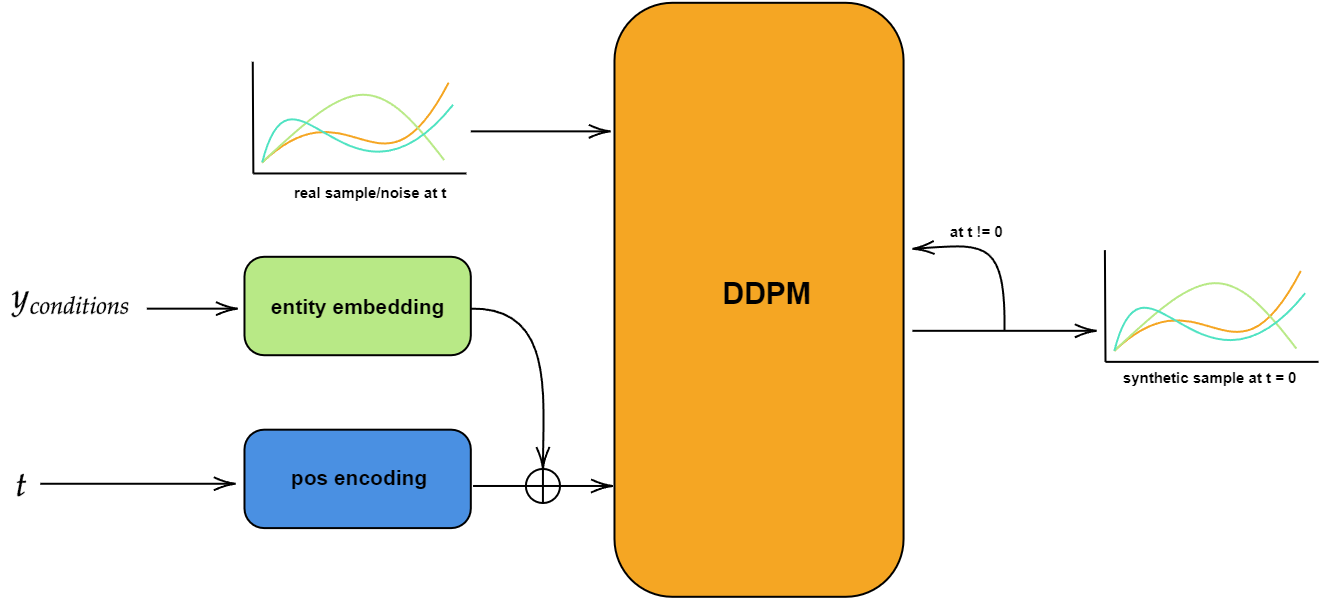
\includegraphics[width=\textwidth]{images/unet1d.png}
    \caption{Visualization of the DDPM process used in this project.}
    \label{fig:unet1d}
\end{figure}
The entire process can be visualized as seen in fig. \ref{fig:unet1d}. The embeddings are simultaneously trained with the model and can be saved and frozen for later usage in other models.
\section{Uni- and Multivariate}
\label{sec: uni and multi}
The until now described architecture are capable of learning/sampling different dimensions of data.
In the field of generative image models this can be easy understood by different color channels. On a more general scale it can be
understood as a multiple target task. The models are trained to synthesize multiple features at the same time. As an example time series data samples are presented. Models that are used in a energy domain mostly focus on some form of "power-delivered" feature they are mostly 
interested in. A univariate model will e.g. now only generate those power time series samples. A Multivariate approach could also 
include learning and synthesizing the temperature and fuel/electricity price time series. In the real world the underlying problem and demand for
a spectrum is bigger so Multivariate approaches seem more attractive. Also they could bring a performance boost by providing more sequential 
context through other features during the training process, which means that the model learns to generate features in relation to and with each other.
These additional features could be already included in the dataset. Examples could be temperature, price of electricity or sun intensity.
But 'virtual' features could be also defined. Such virtual features could be a daily sine or cosine graph that maps a single timestamp in a day to a tuple of sine/cosine values.
For better understanding a sample was taken from an experiment defined at section \ref{sec:experiments}. In figure \ref{fig:multivar example} you can see a real featuer kW and two virtual ones.
\begin{figure}[h!]
    \centering
    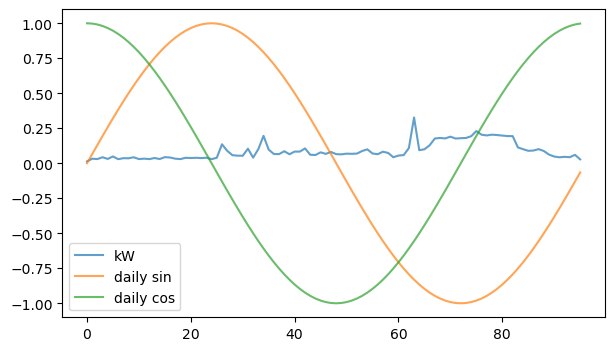
\includegraphics[width=0.6\textwidth]{images/multivar_example.png}
    \caption{A multivariate sample containing kW,daily sin and daily cos as dimensions.}
    \label{fig:multivar example}
\end{figure}
